\documentclass[aspectratio=169]{beamer}

\usetheme{Madrid}
\usecolortheme{default}
\setbeamertemplate{navigation symbols}{}
\setbeamertemplate{headline}{}
\setbeamertemplate{footline}[frame number]

\usepackage{graphicx}
\usepackage{booktabs}
\usepackage{listings}
\usepackage{xcolor}
\usepackage{hyperref}

\lstset{
  basicstyle=\ttfamily\scriptsize,
  backgroundcolor=\color{gray!10},
  frame=single,
  breaklines=true,
  showstringspaces=false,
  tabsize=2
}

\title{UrbanMove Smart Mobility on AWS}
\subtitle{Cloud Computing Final Lab}
\author{Jordy Meye \and Huizhe Su \and Arihant Jain \and Nizar}
\institute{EPITA -- Master in Computer Science}
\date{April 2026}

\begin{document}

\begin{frame}
  \titlepage
\end{frame}

\begin{frame}{Agenda}
  \tableofcontents
\end{frame}

\section{Scope}
\begin{frame}{Project Scope}
  \begin{itemize}
    \item Build and deploy a 3-service mobility platform.
    \item Keep service runtime in private subnets.
    \item Route API traffic through CloudFront and API Gateway.
    \item Add IAM baseline, WAF, monitoring, and cost controls.
    \item Deliver report, evidence, and demo-ready UI.
  \end{itemize}
\end{frame}

\section{Architecture}
\begin{frame}{Final Architecture}
  \centering
  
\includegraphics[width=\textwidth,height=0.78\textheight,keepaspectratio]{../architecture/exports/architecture_design.png}
\end{frame}

\begin{frame}{Runtime Components}
  \begin{tabular}{p{0.26\textwidth}p{0.67\textwidth}}
    \toprule
    \textbf{Component} & \textbf{Role} \\
    \midrule
    urbanmove-api & REST facade, request validation, calls auth and routing via gRPC \\
    urbanmove-auth & JWT issue and validation, role checks \\
    urbanmove-ingestion-routing & Gov feed ingestion, simulator fallback, route logic \\
    PostgreSQL + NATS & Data persistence and messaging backbone \\
    Bastion host & SSH jump host for private instances \\
    \bottomrule
  \end{tabular}
\end{frame}

\section{Security and Networking}
\begin{frame}{Network and Security Controls}
  \begin{itemize}
    \item CloudFront default origin: S3 frontend bucket.
    \item CloudFront \texttt{/api/*} origin: API Gateway.
    \item API Gateway private integration: VPC Link to internal NLB.
    \item Services run in private subnets; outbound only through NAT Gateway.
    \item WAF Web ACL associated with CloudFront distribution.
    \item IAM setup includes deploy identity and EC2 instance role/profile.
  \end{itemize}
\end{frame}

\begin{frame}{Infrastructure Evidence: Network}
  \begin{columns}[T]
    \column{0.5\textwidth}
    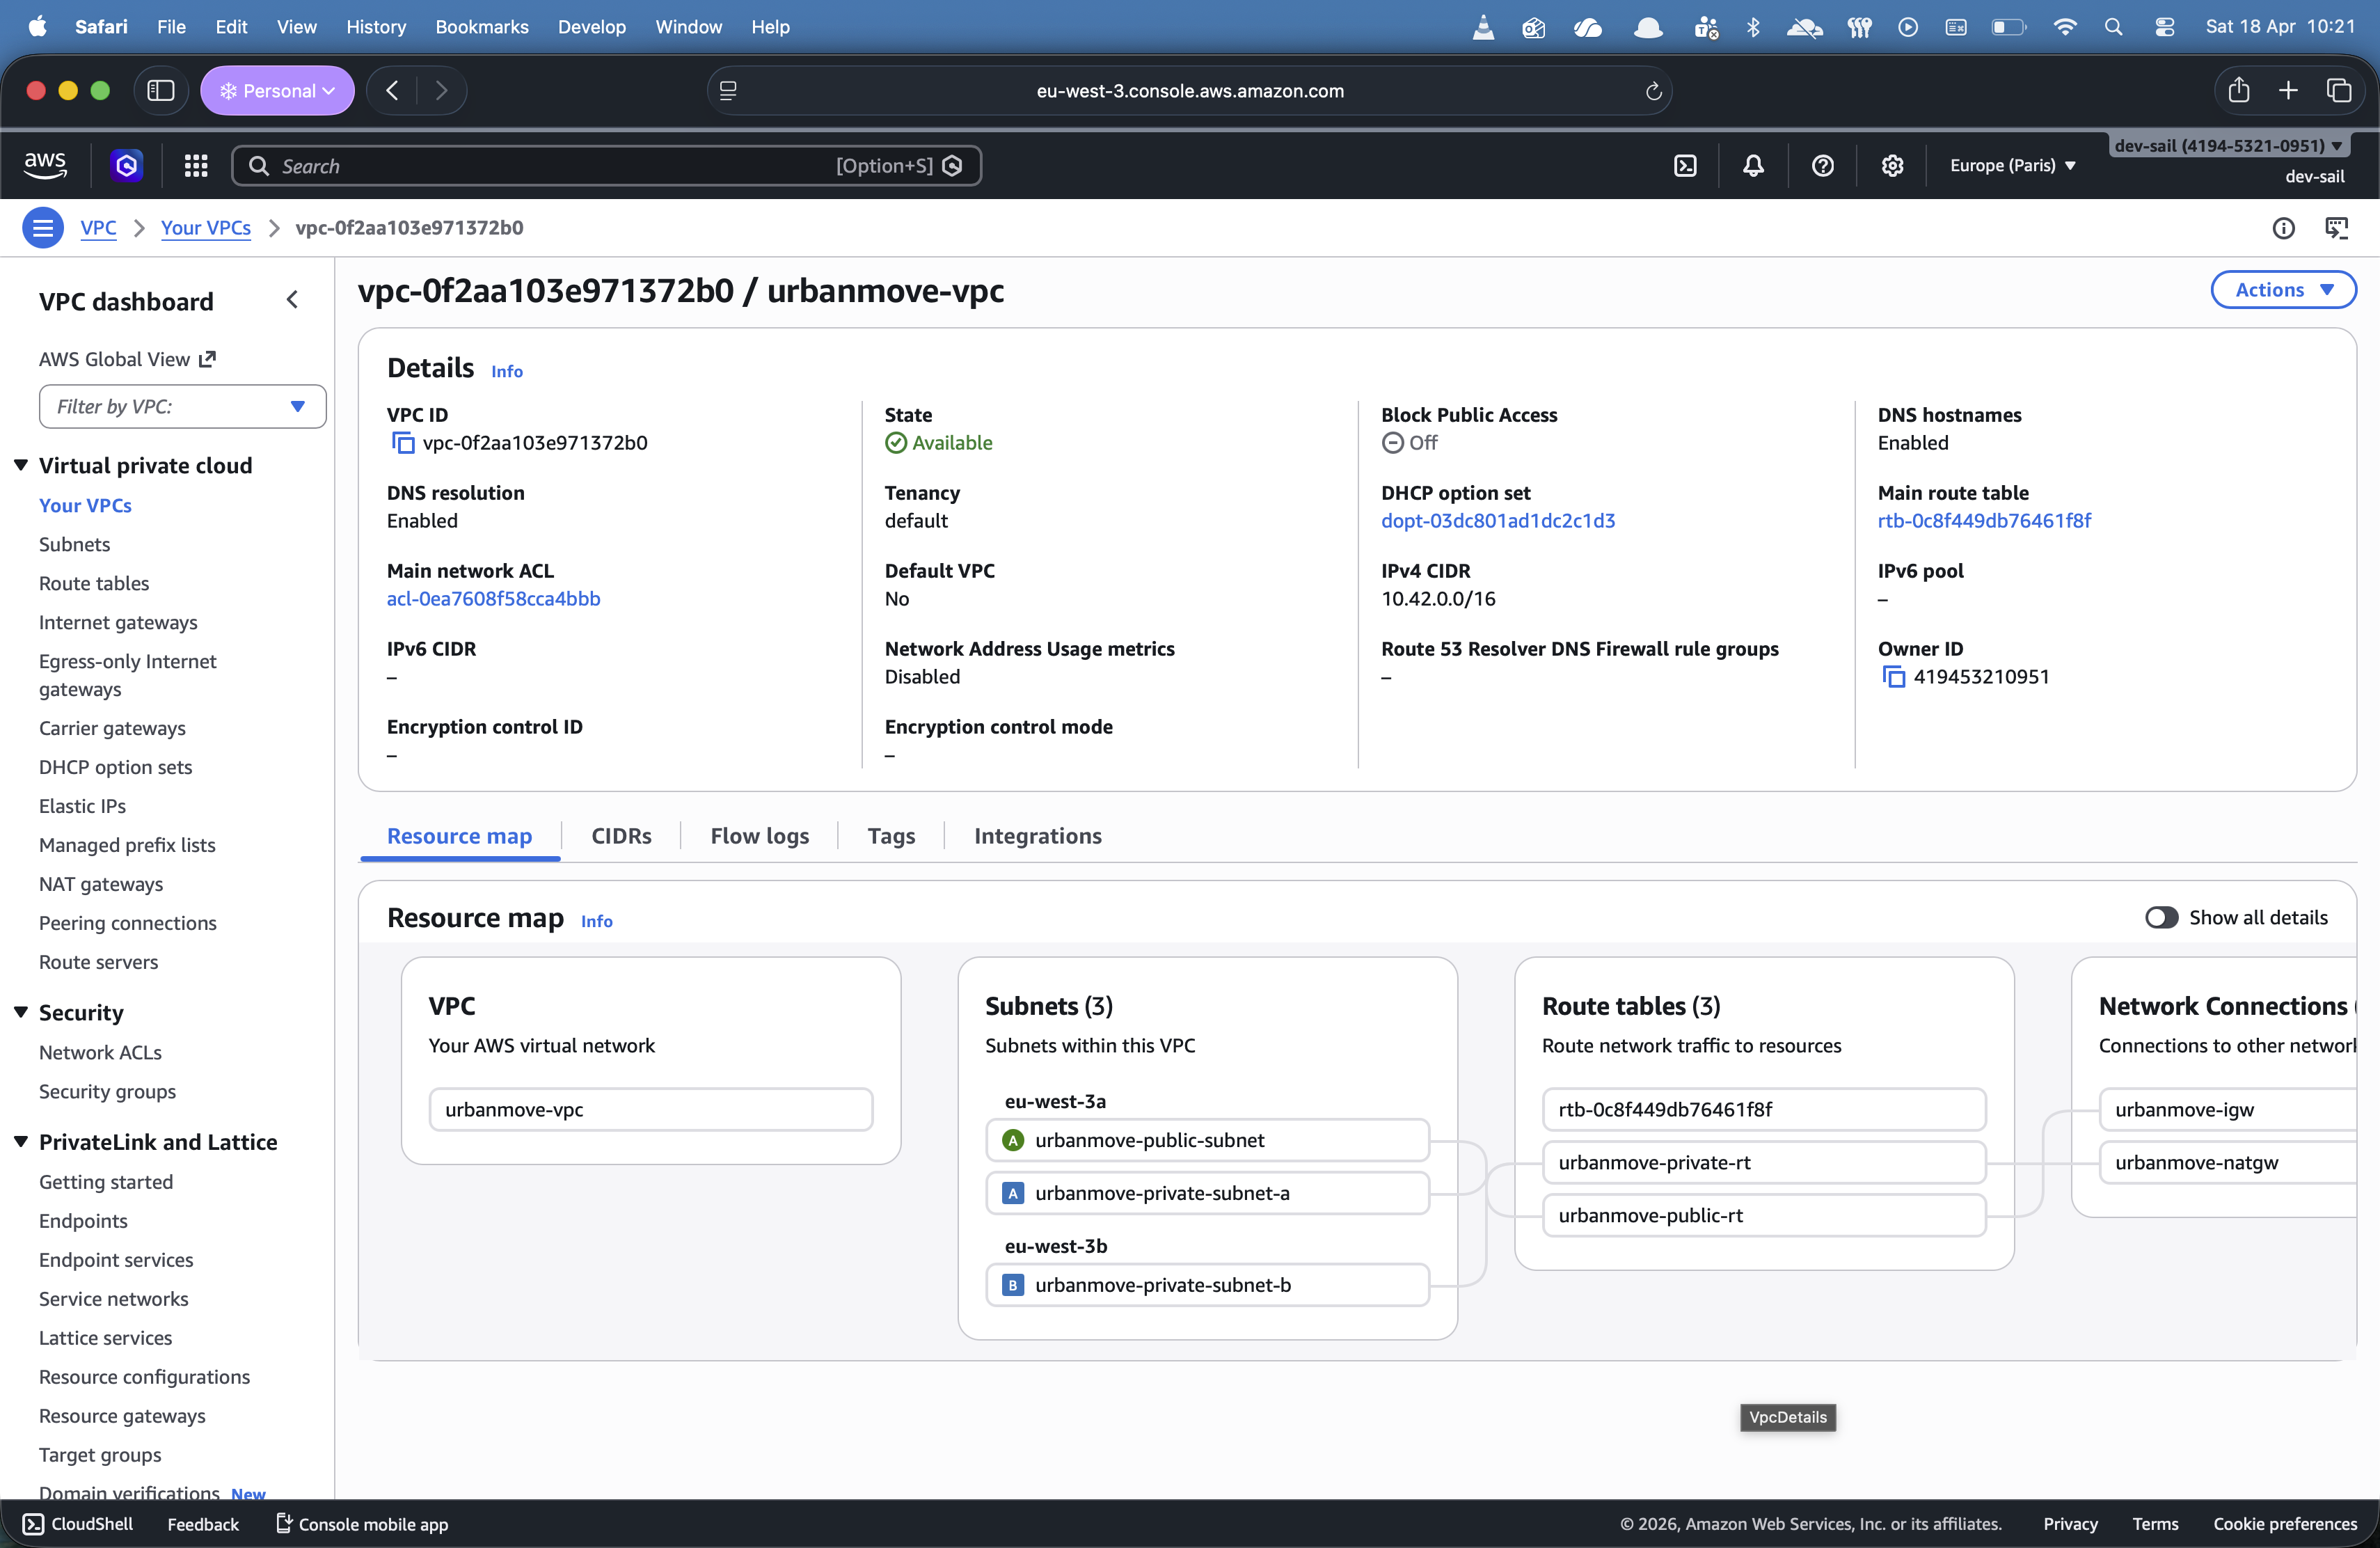
\includegraphics[width=\textwidth,height=0.70\textheight,keepaspectratio]{../evidence/screenshots/02-infra/vpc_with_subnets_and_routes.png}
    \column{0.5\textwidth}
    
\includegraphics[width=\textwidth,height=0.70\textheight,keepaspectratio]{../evidence/screenshots/02-infra/nat_gateway.png}
  \end{columns}
\end{frame}

\begin{frame}{Infrastructure Evidence: Edge and Compute}
  \begin{columns}[T]
    \column{0.5\textwidth}
    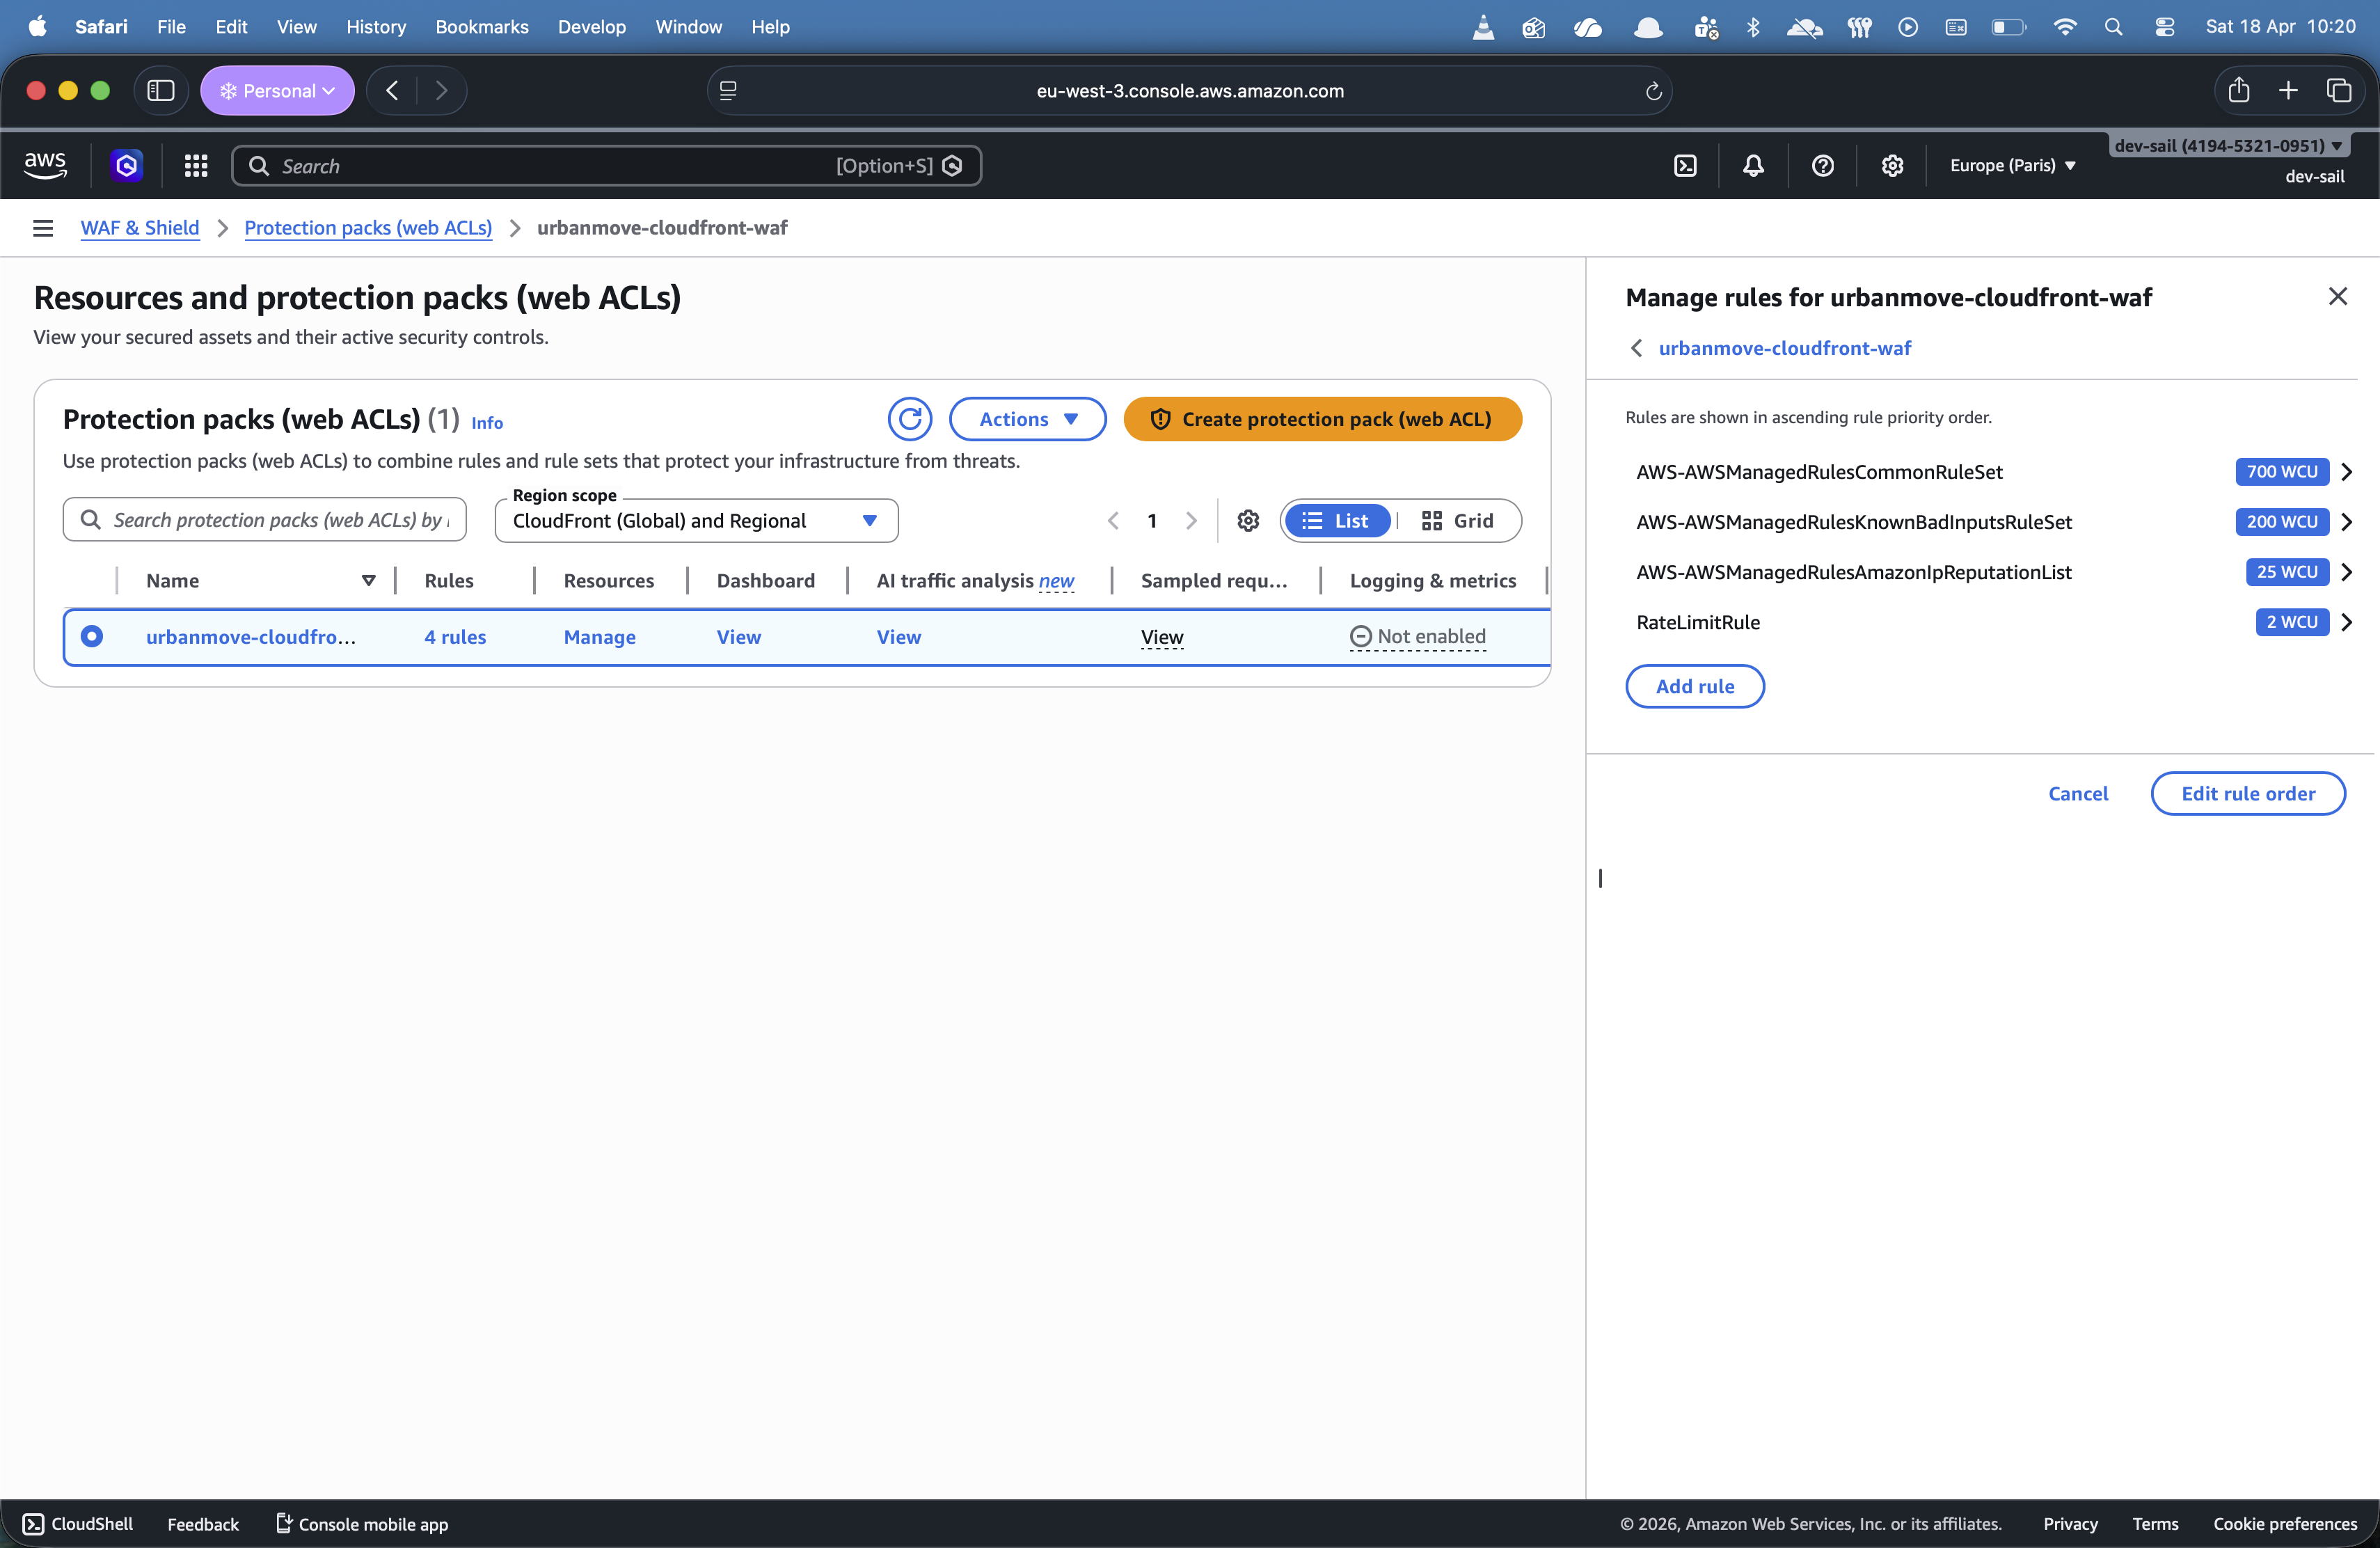
\includegraphics[width=\textwidth,height=0.70\textheight,keepaspectratio]{../evidence/screenshots/02-infra/waf.png}
    \column{0.5\textwidth}
    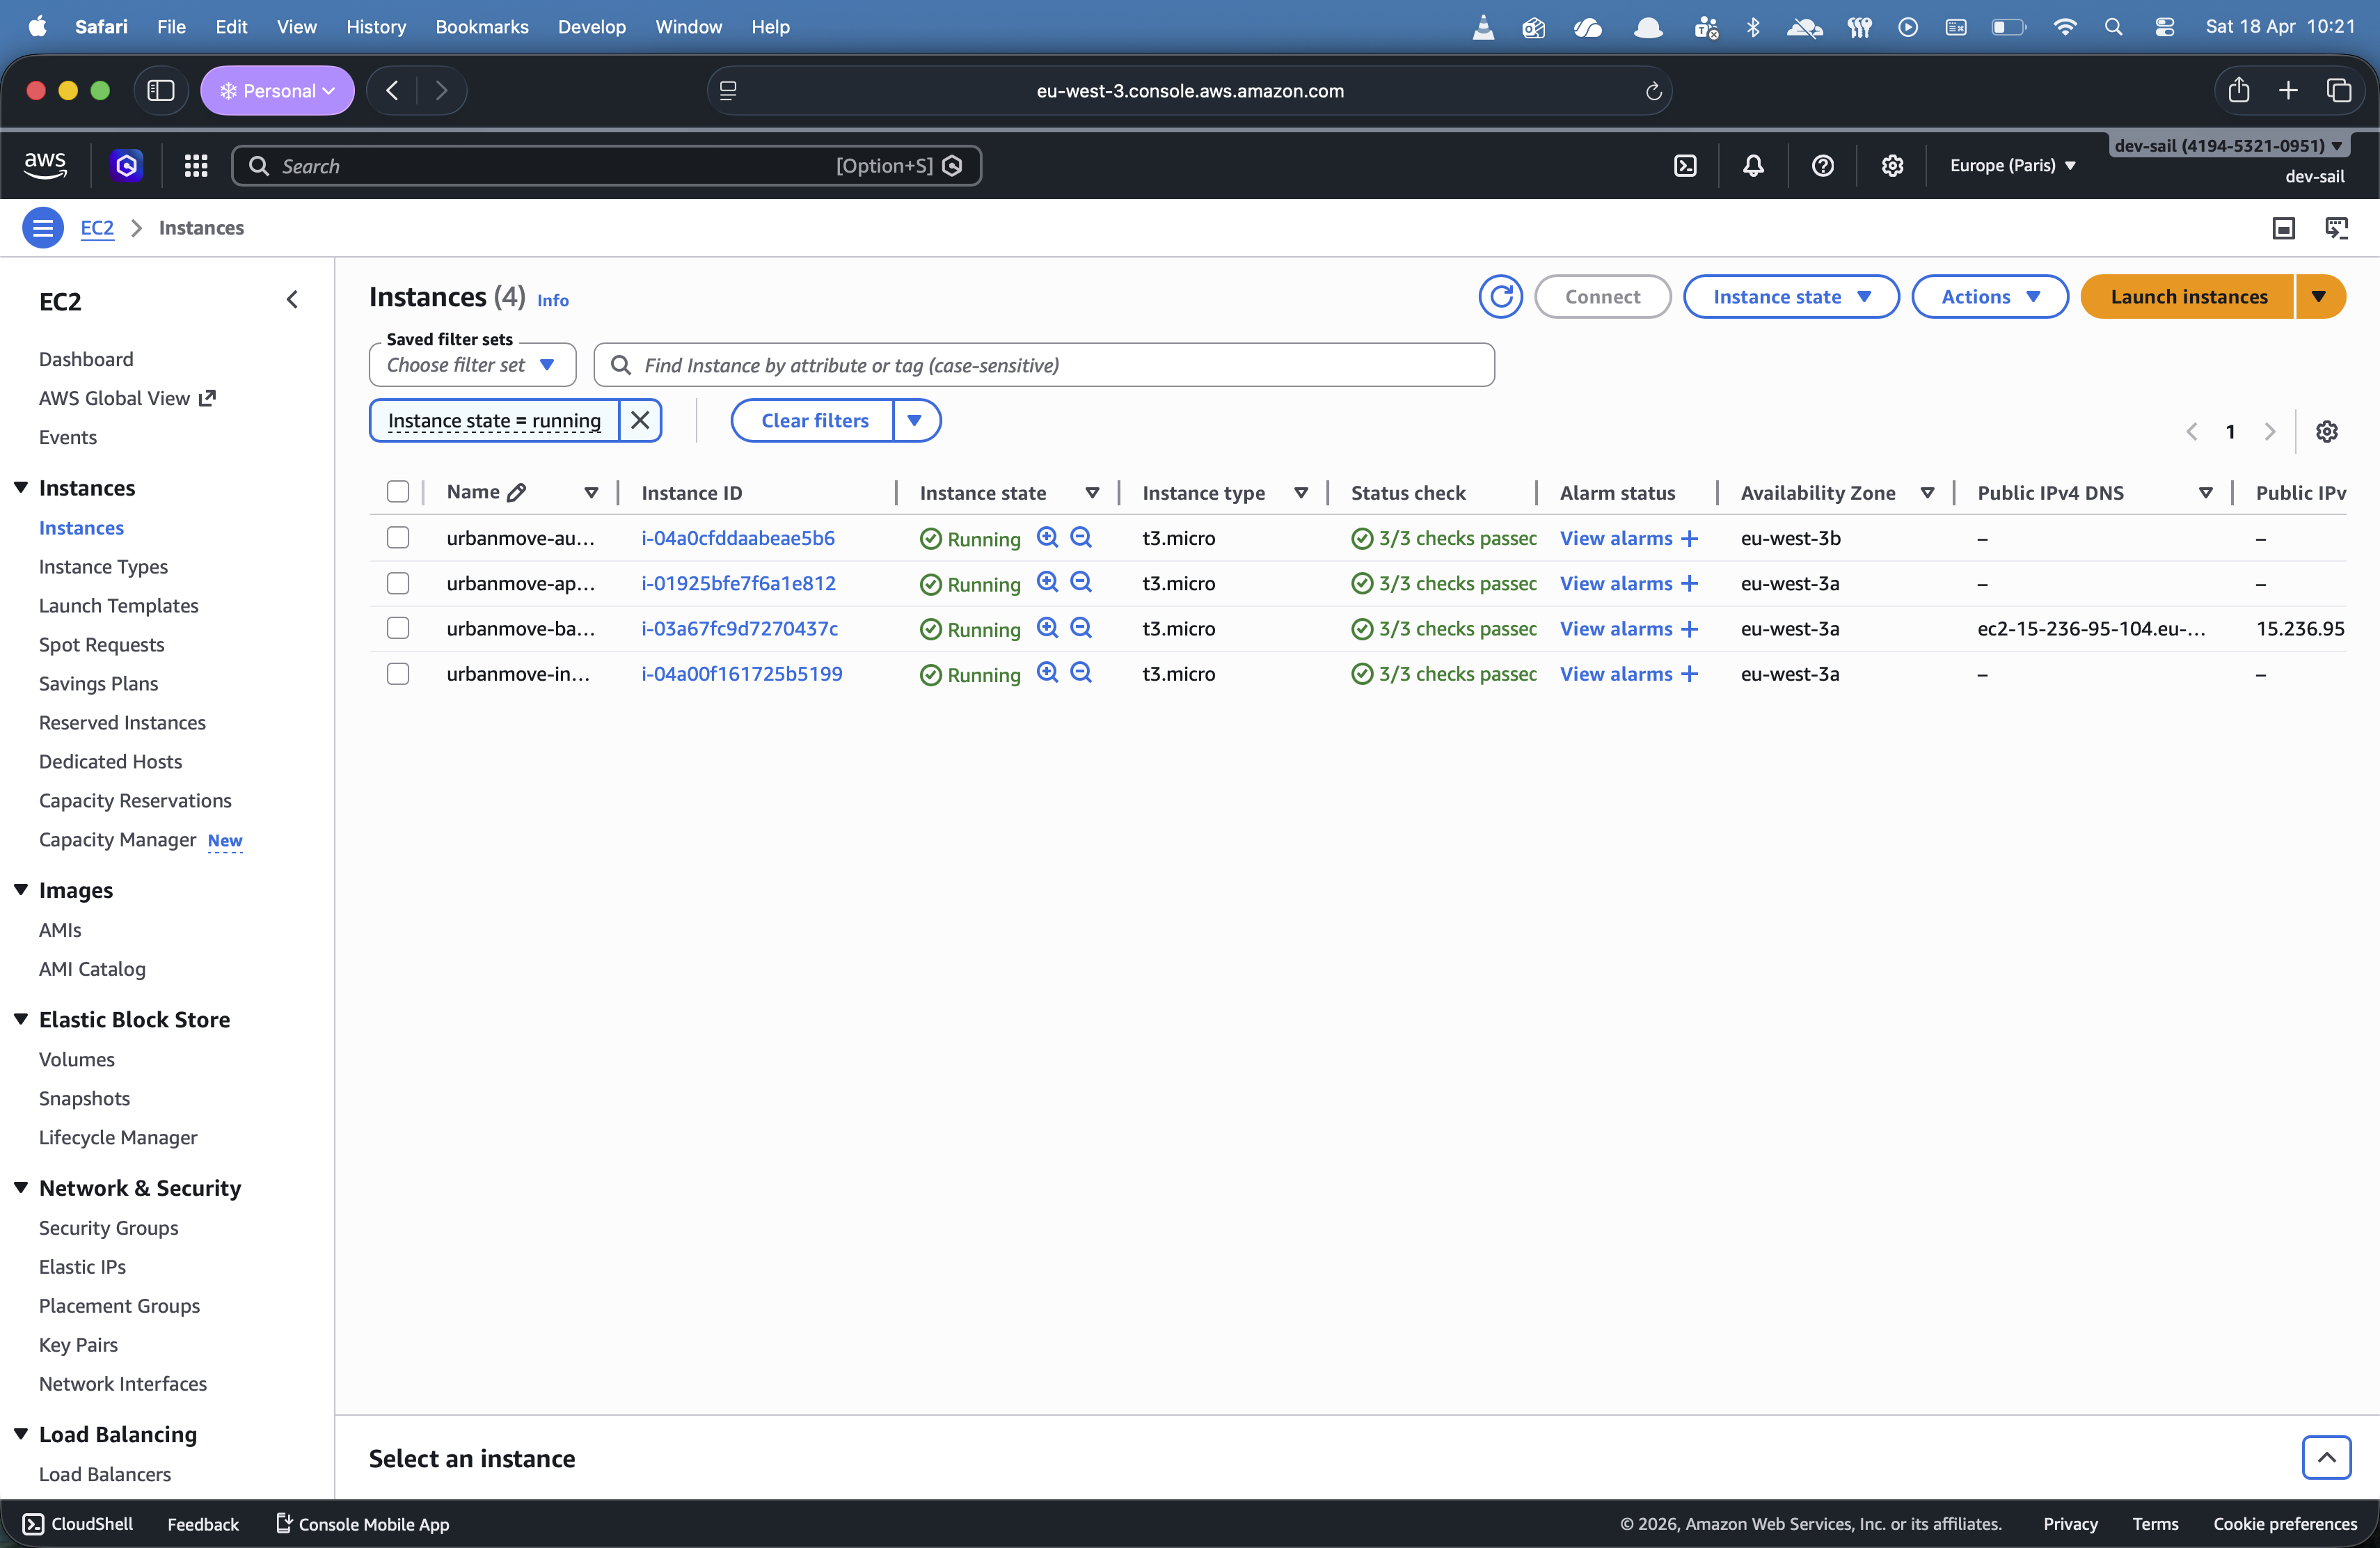
\includegraphics[width=\textwidth,height=0.70\textheight,keepaspectratio]{../evidence/screenshots/02-infra/ec2_instances.png}
  \end{columns}
\end{frame}

\section{Automation}
\begin{frame}[fragile]{Infra Provisioning Script Sequence}
\begin{lstlisting}[language=bash]
cd lab_final/infra/aws-cli
./01_budget_and_tags.sh
./01a_identity_iam_setup.sh
./02a_create_vpc_private_network.sh
./02_create_ec2_topology.sh
./03a_api_gateway_setup.sh
./03_s3_cloudfront_setup.sh
./04_cloudwatch_setup.sh
./06_waf_setup.sh
\end{lstlisting}
\end{frame}

\begin{frame}[fragile]{Deployment Script Sequence}
\begin{lstlisting}[language=bash]
cd lab_final/infra/deploy
./01_bootstrap_hosts.sh
./02_deploy_auth.sh
./03_deploy_ingest.sh
./04_deploy_api.sh
./05_upload_frontend.sh
./06_smoke_test.sh
\end{lstlisting}
\end{frame}

\section{Application Flow}
\begin{frame}{API Flow Evidence}
  \centering
  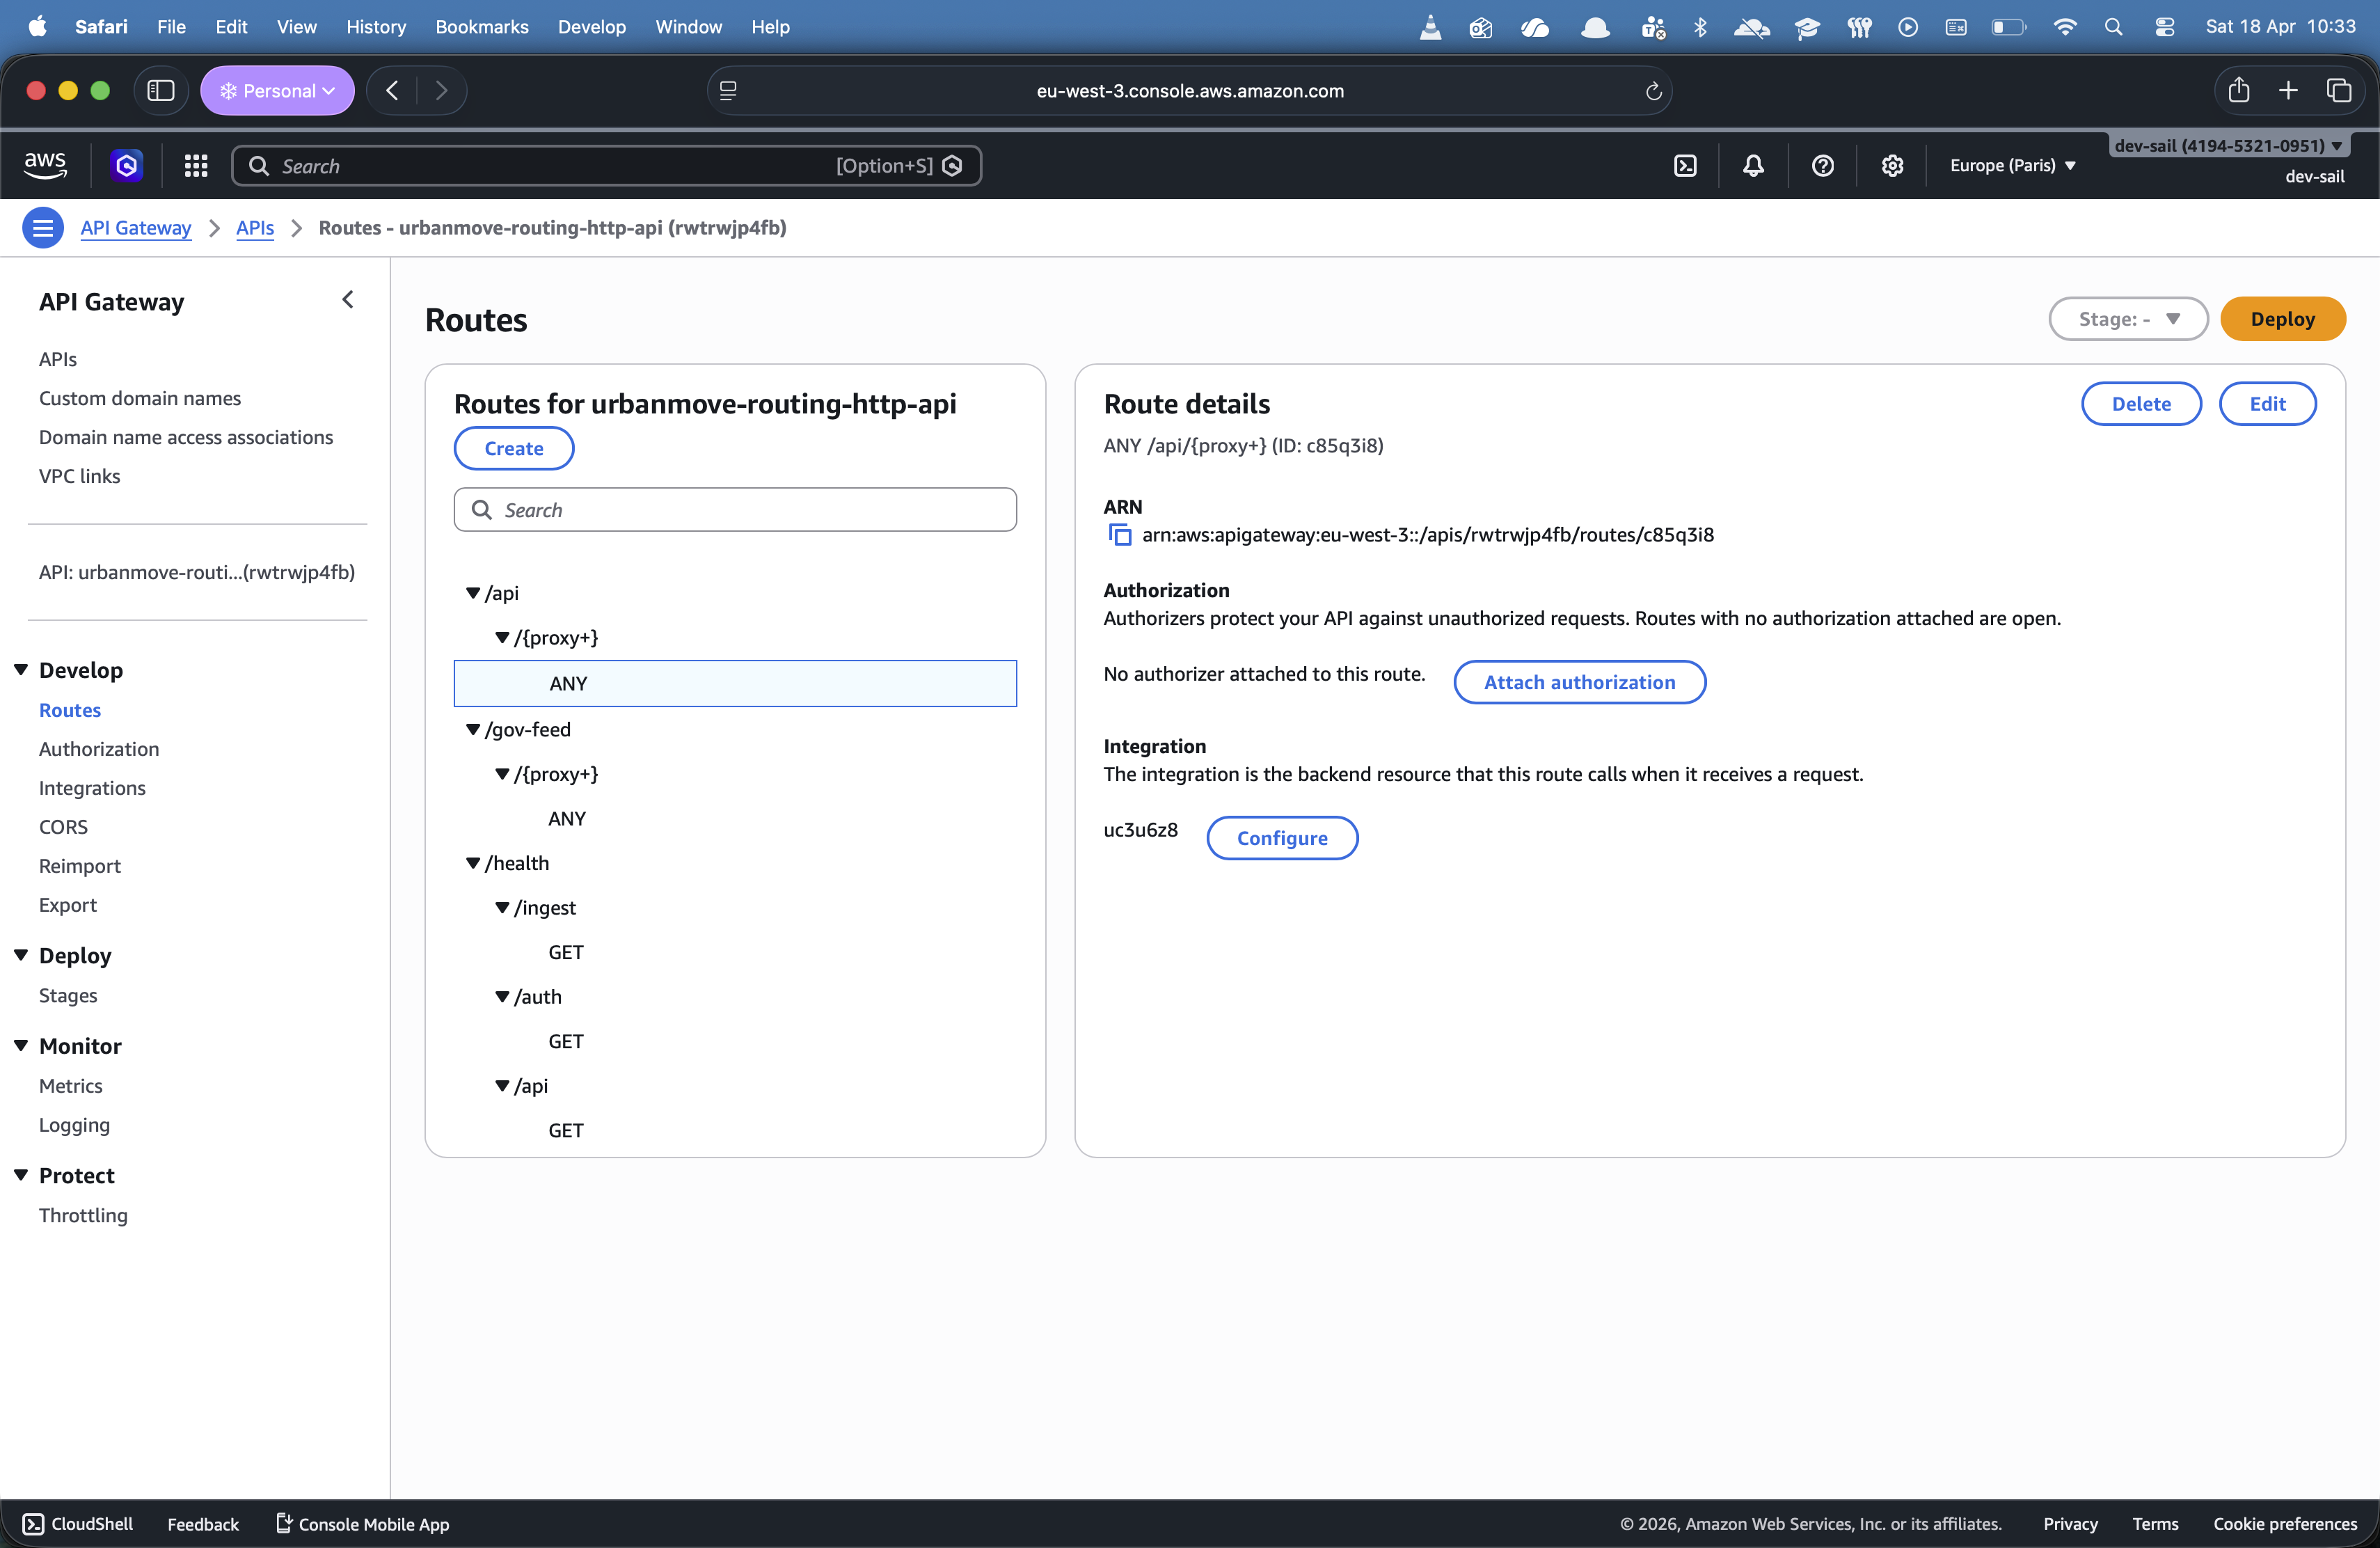
\includegraphics[width=\textwidth,height=0.75\textheight,keepaspectratio]{../evidence/screenshots/04-api-flow/api_gateway_routes.png}
\end{frame}

\begin{frame}{Frontend Flow}
  \begin{columns}[T]
    \column{0.5\textwidth}
    \textbf{Login page}\\[0.3em]
    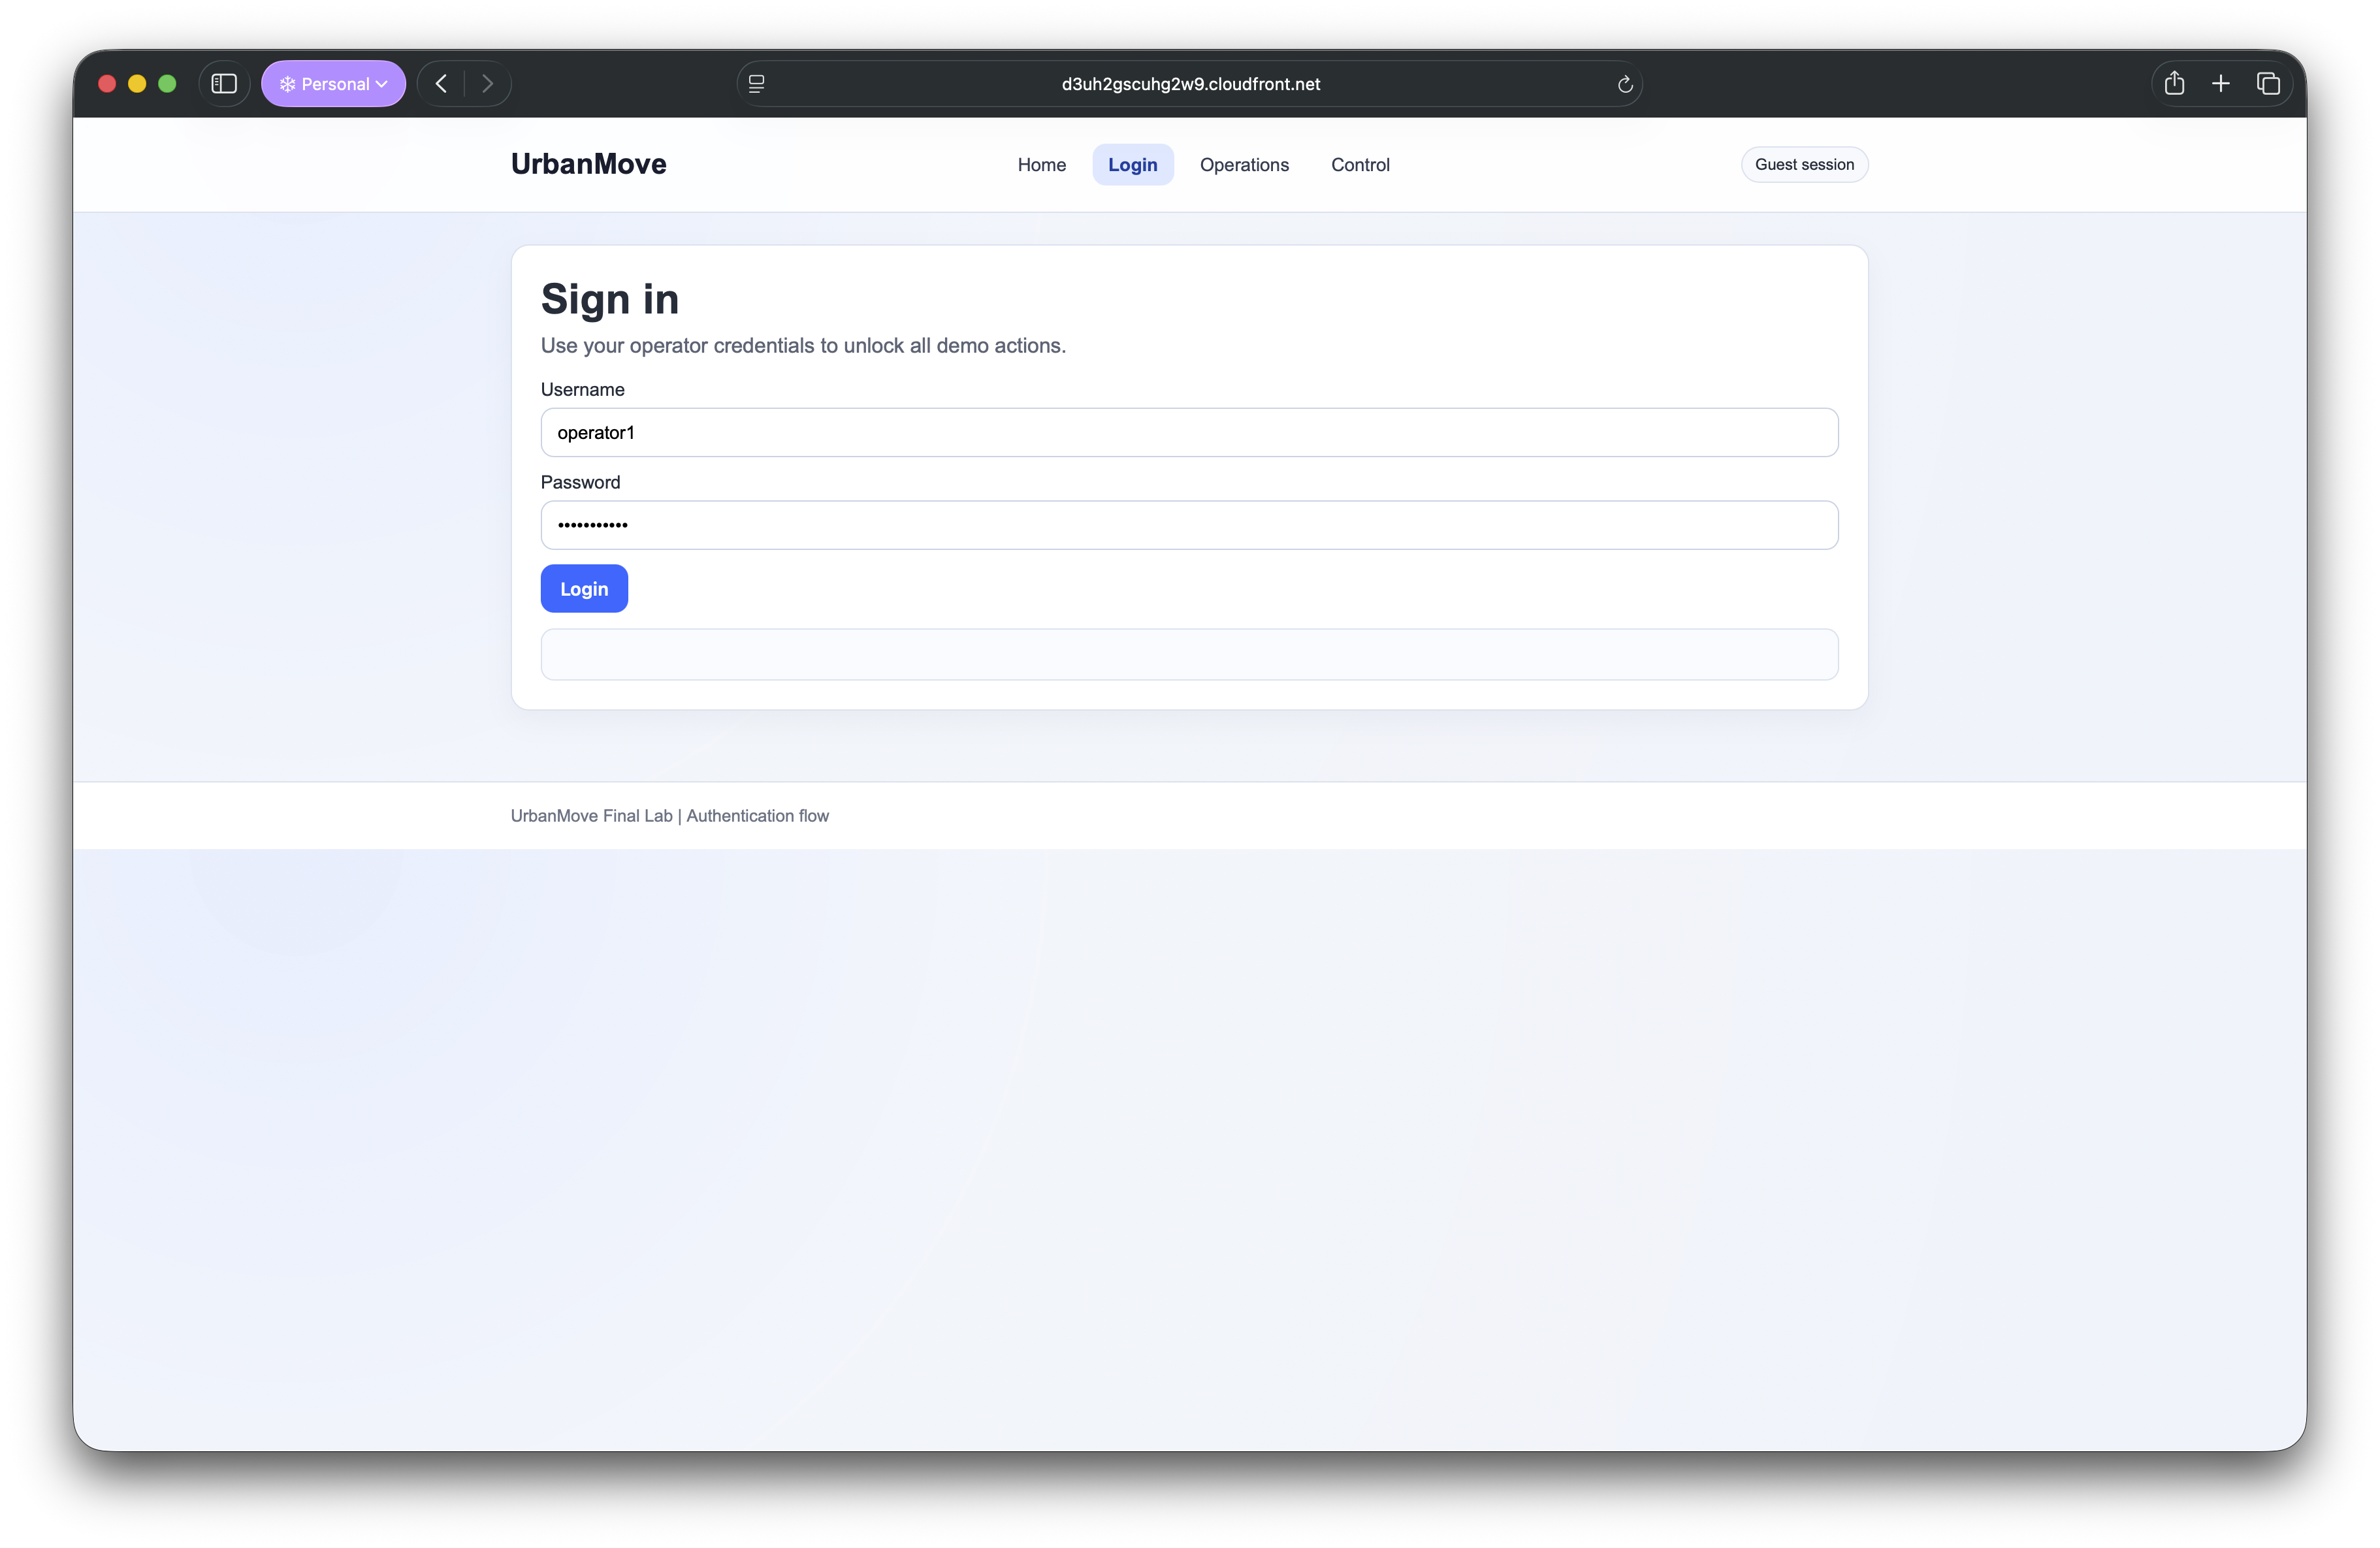
\includegraphics[width=\textwidth]{../evidence/screenshots/04-api-flow/frontend_login.png}
    \column{0.5\textwidth}
    \textbf{Operations and control pages}\\[0.3em]
    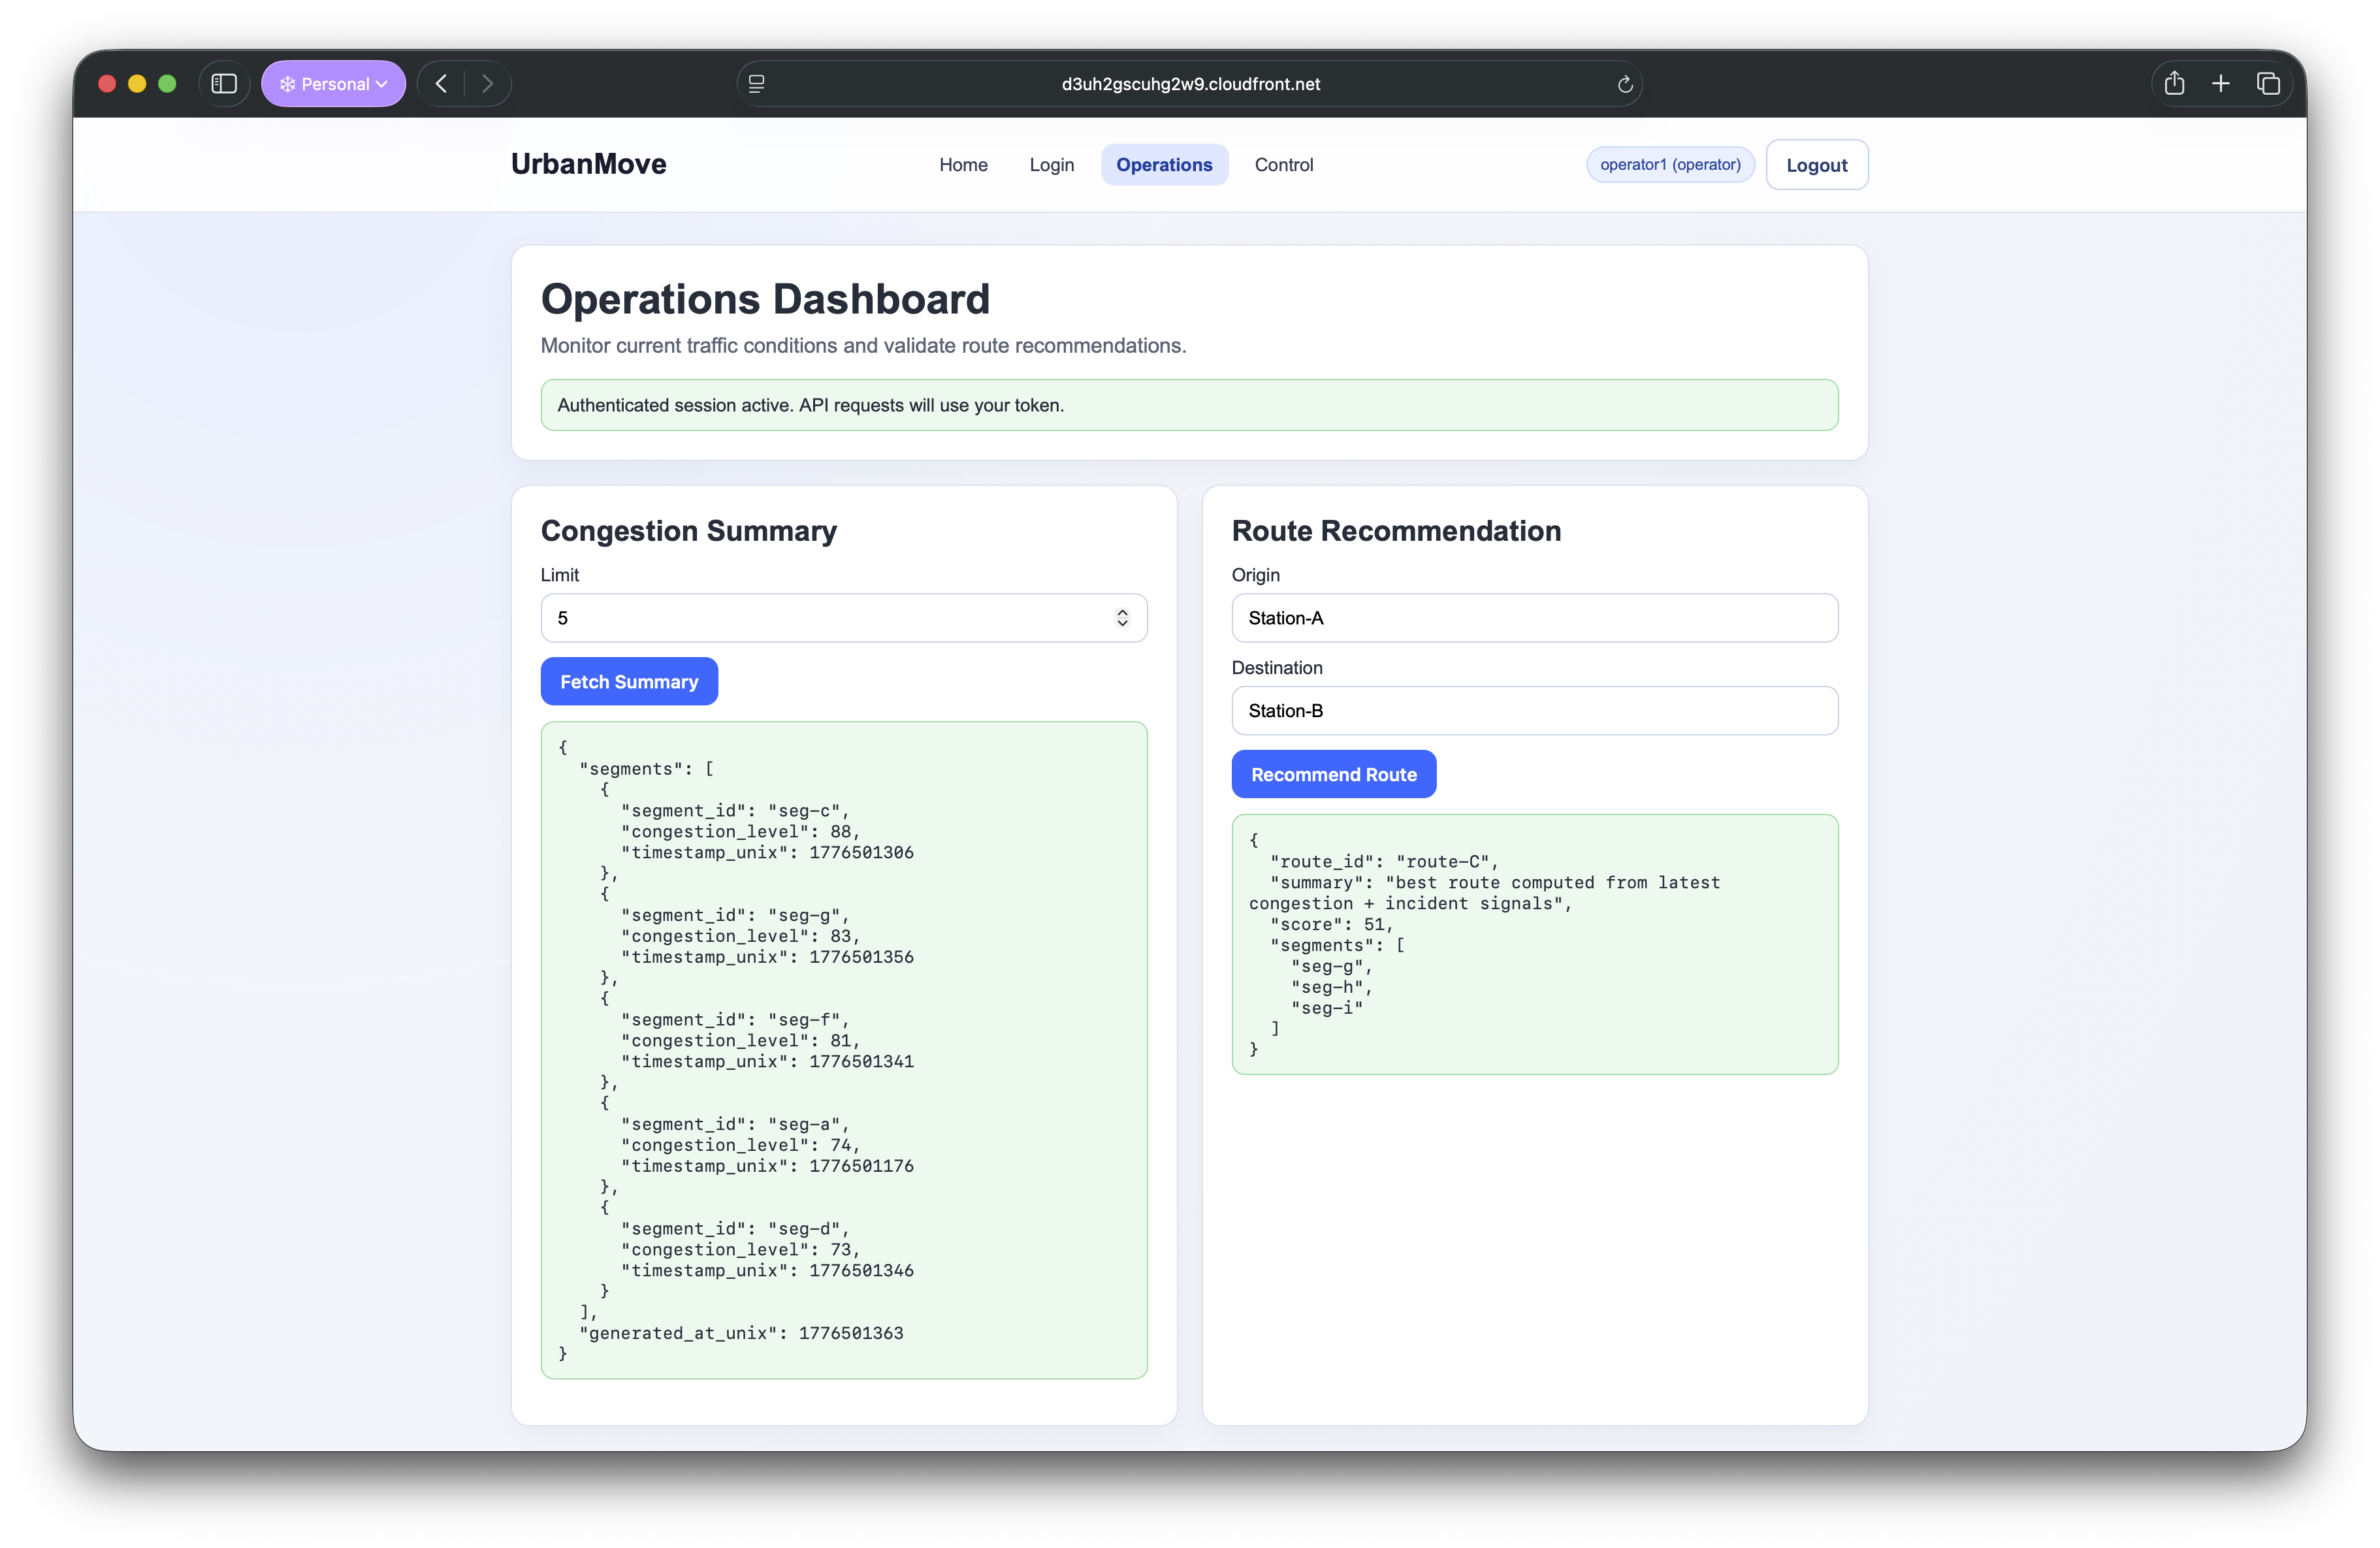
\includegraphics[width=\textwidth]{../evidence/screenshots/04-api-flow/frontend_operations.png}
  \end{columns}
\end{frame}

\begin{frame}{End-to-End Validation}
  \centering
  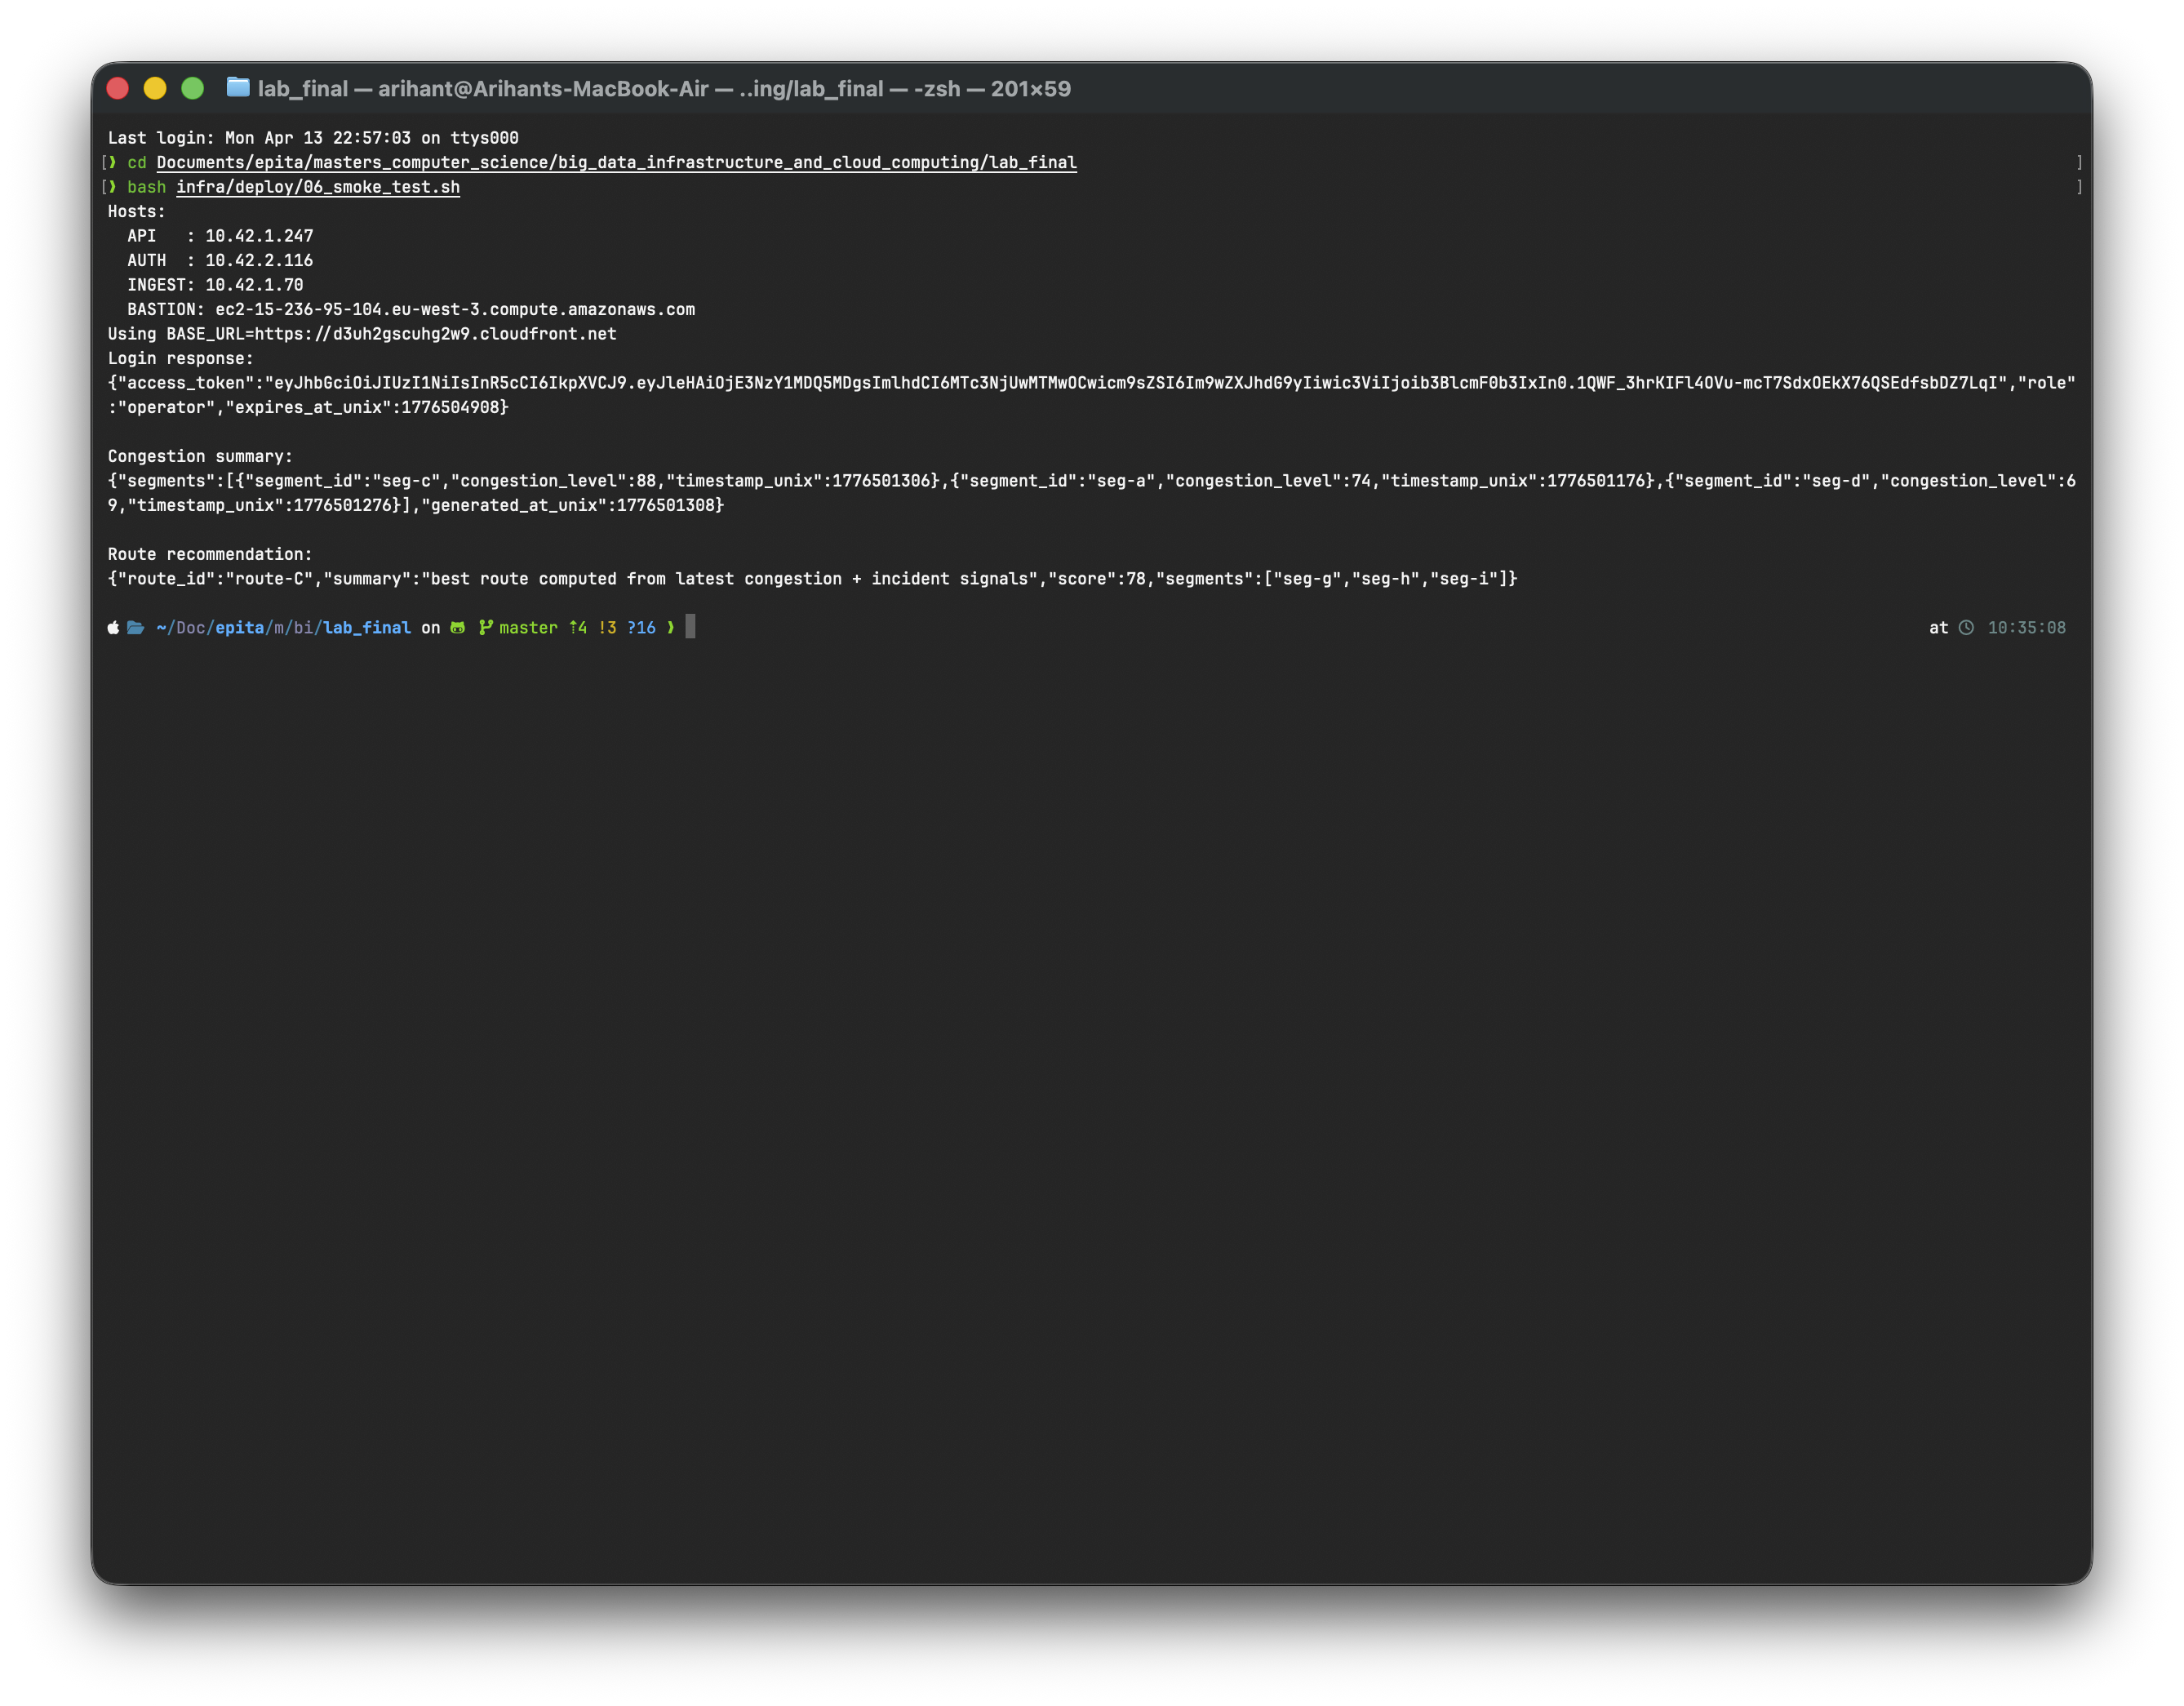
\includegraphics[width=\textwidth,height=0.75\textheight,keepaspectratio]{../evidence/screenshots/04-api-flow/smoke_test_success.png}
\end{frame}

\section{Operations}
\begin{frame}{Monitoring and Budget Evidence}
  \begin{columns}[T]
    \column{0.5\textwidth}
    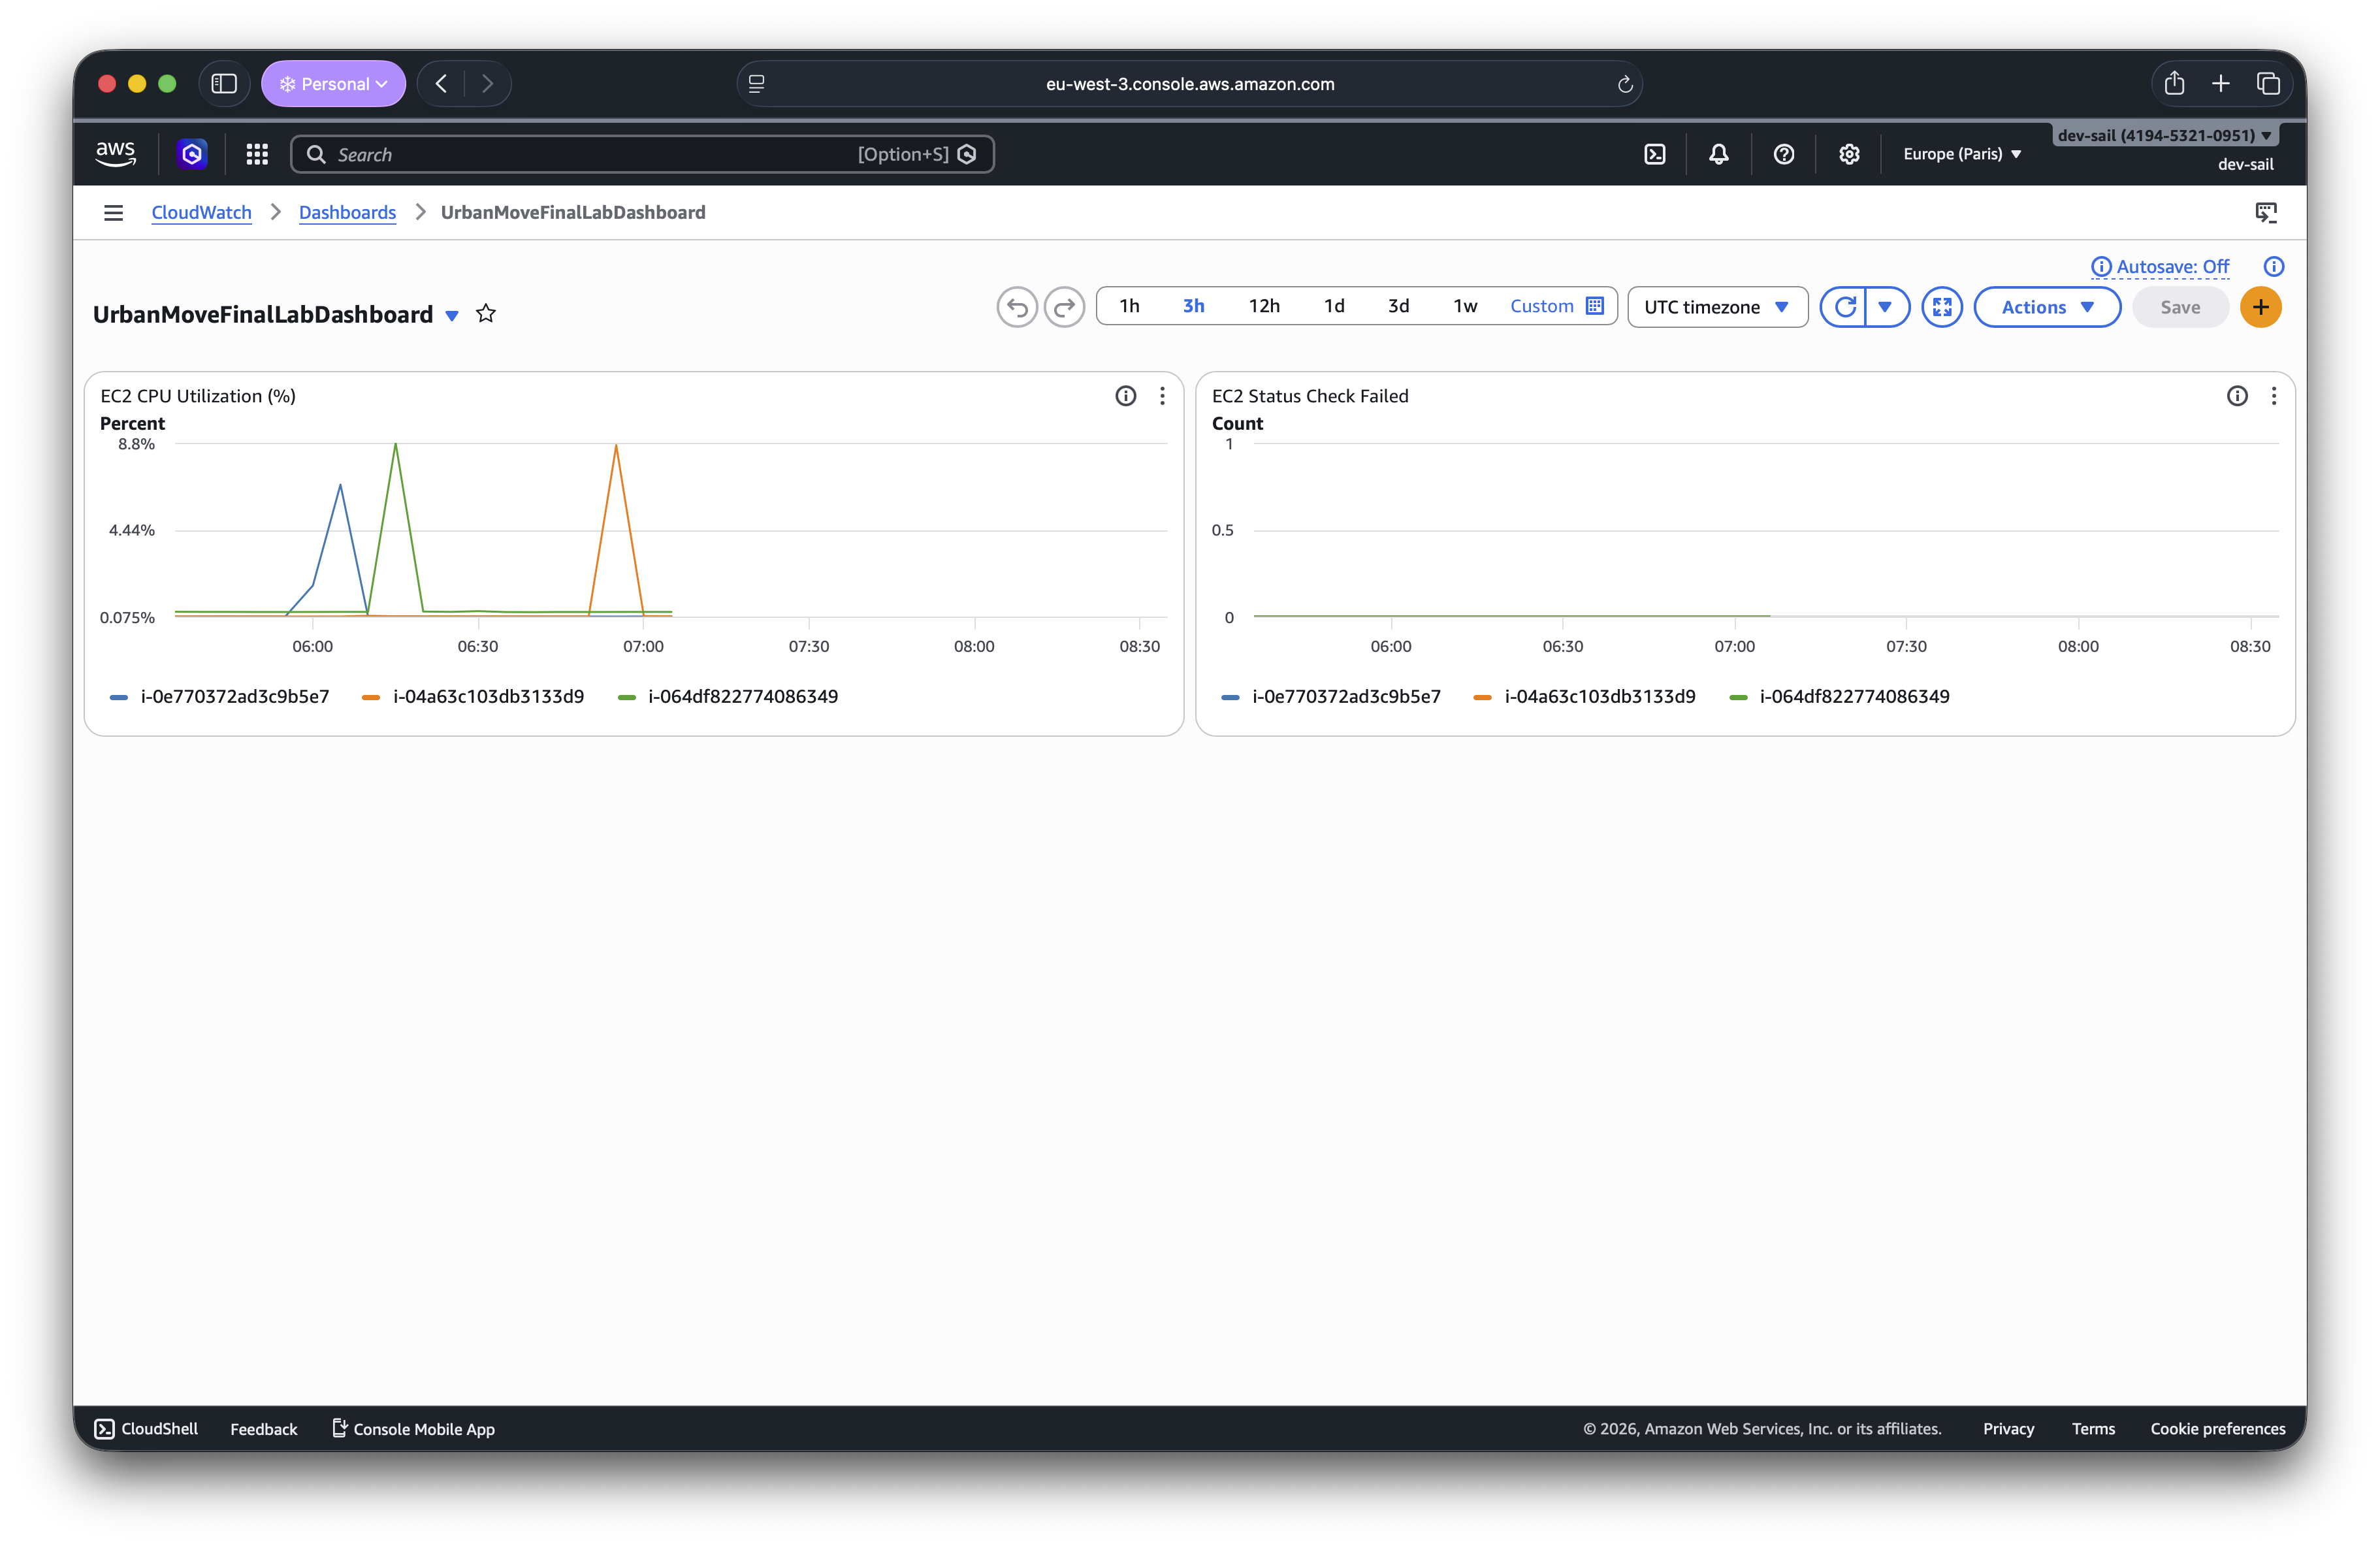
\includegraphics[width=\textwidth,height=0.70\textheight,keepaspectratio]{../evidence/screenshots/05-observability/cloudwatch_dashboard.png}
    \column{0.5\textwidth}
    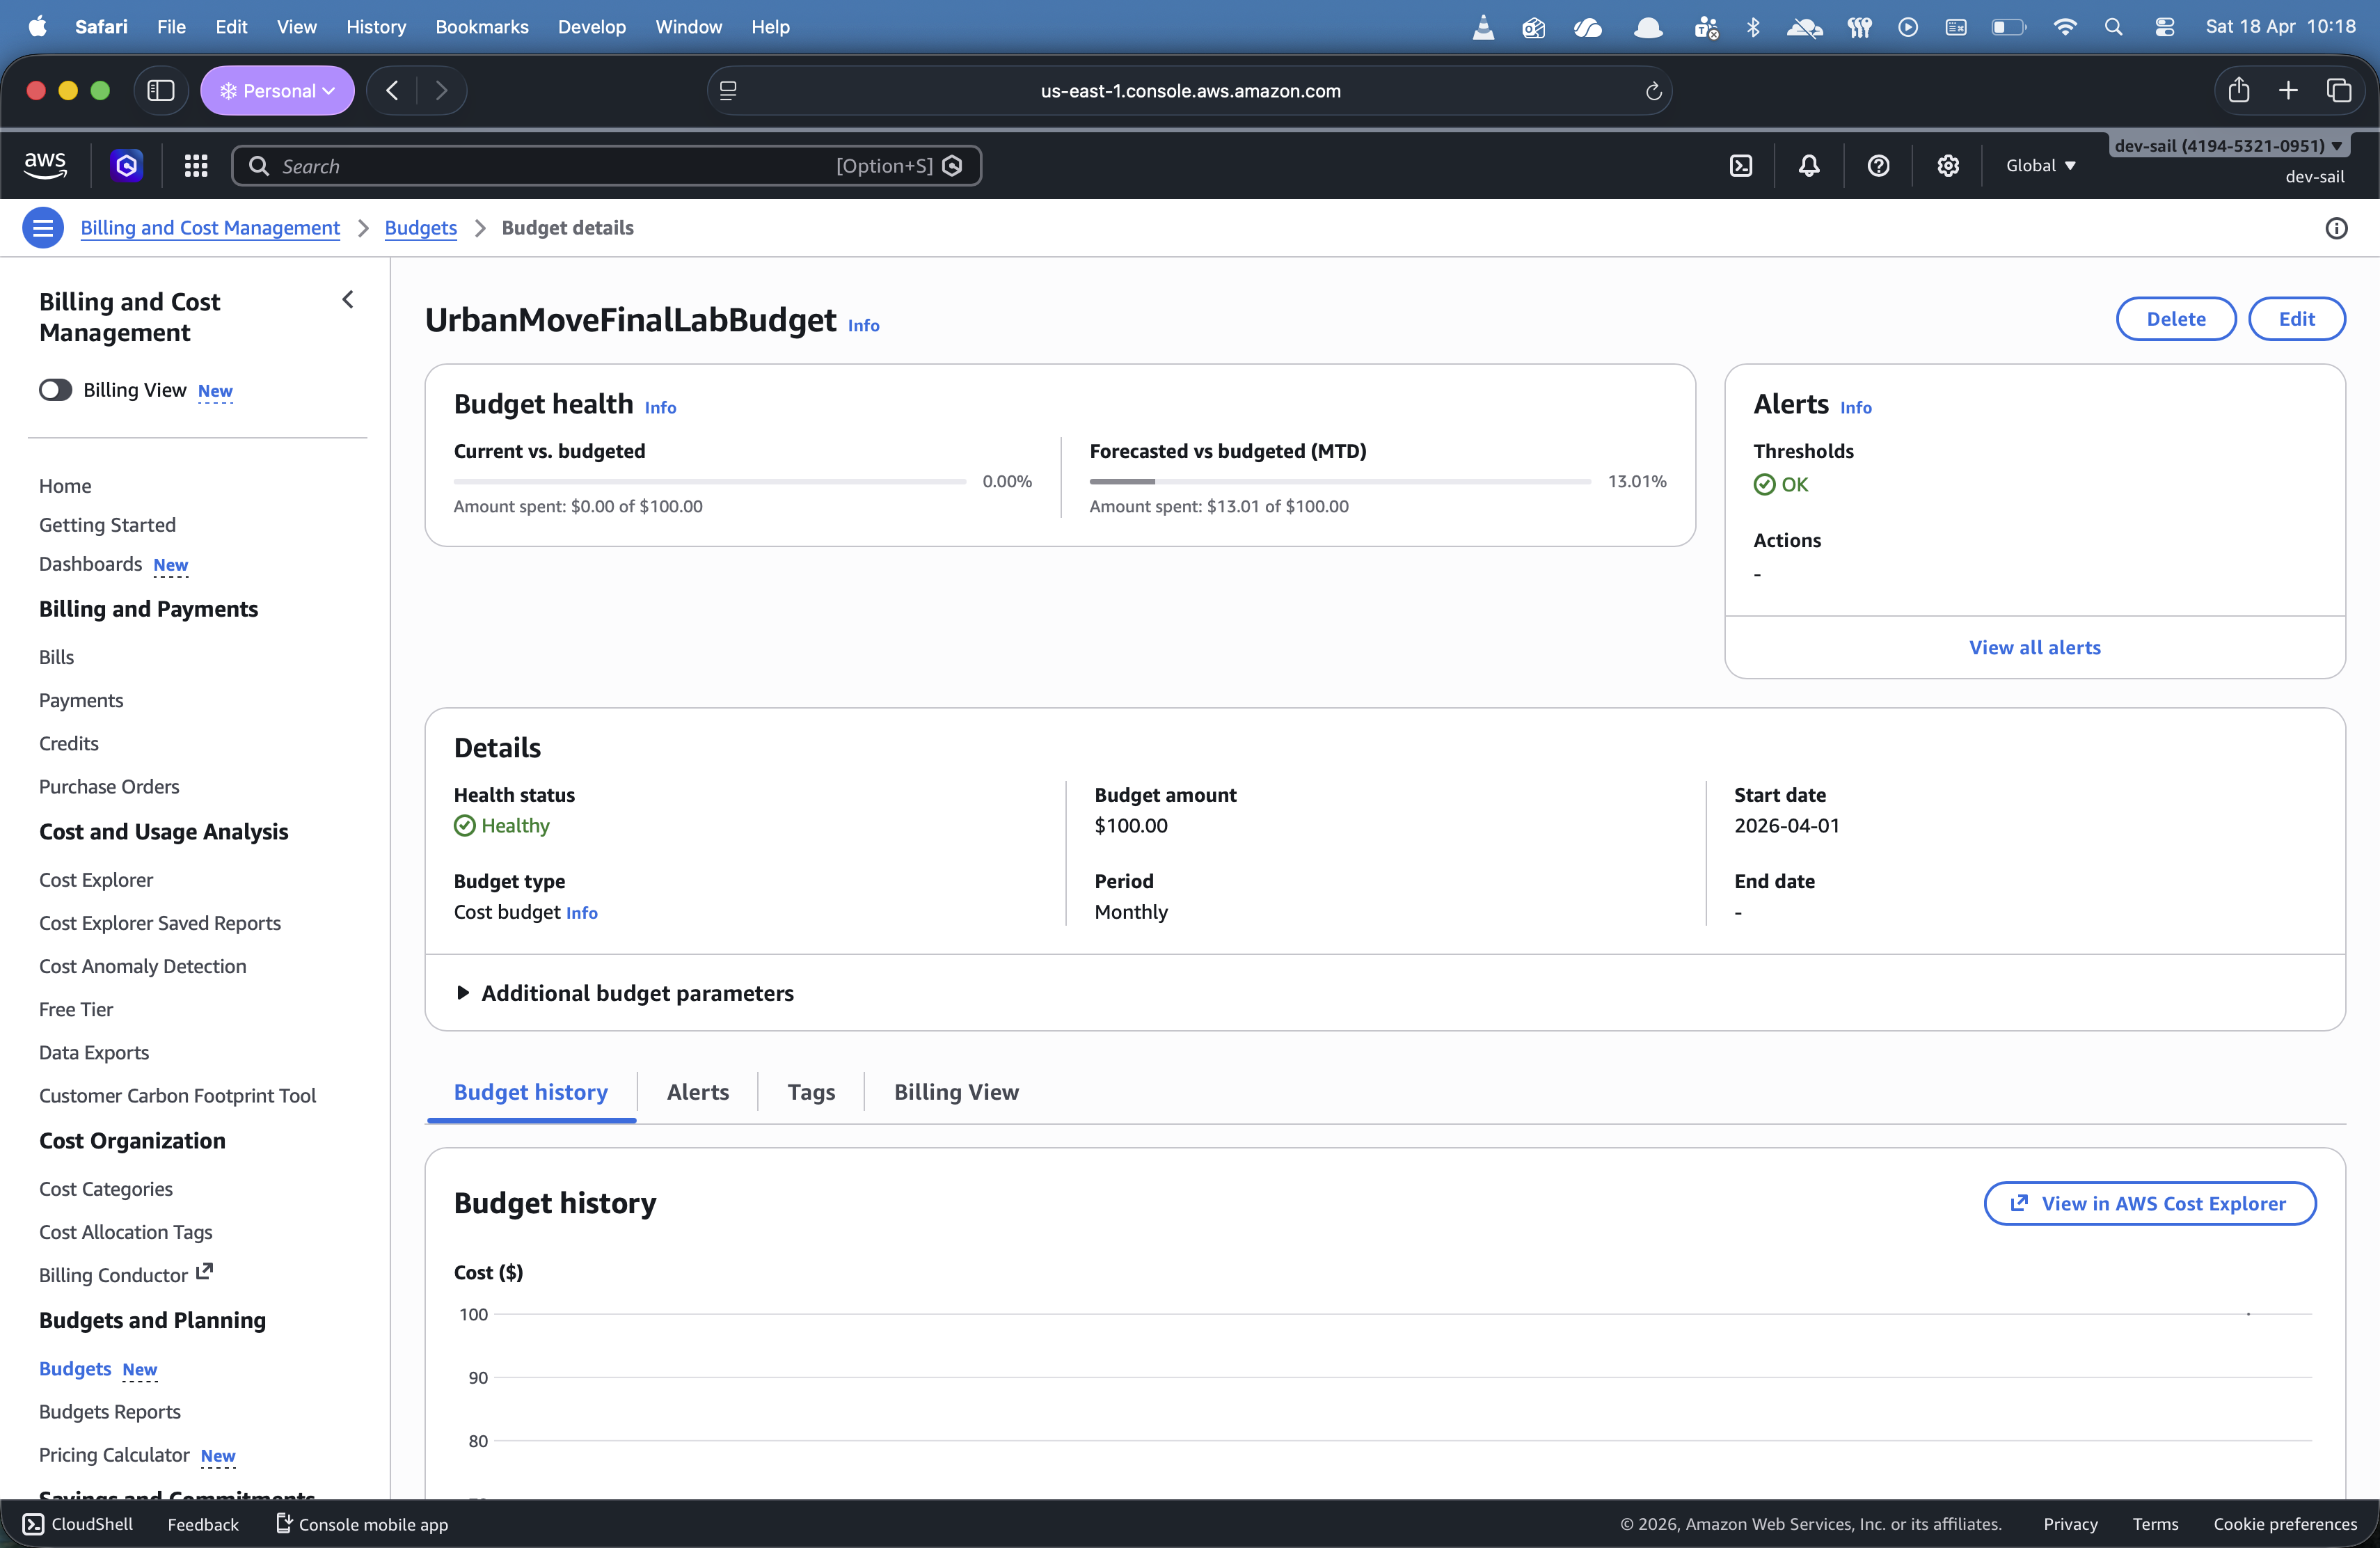
\includegraphics[width=\textwidth,height=0.70\textheight,keepaspectratio]{../evidence/screenshots/01-budget/budget.png}
  \end{columns}
\end{frame}

\begin{frame}[fragile]{Backup and Restore Drill (Non-Destructive)}
\begin{lstlisting}[language=bash]
# on ingest host
sudo docker exec urbanmove-postgres \
  pg_dump -U urbanmove -d urbanmove > /tmp/urbanmove_backup.sql

sudo docker exec -i urbanmove-postgres psql -U urbanmove -d postgres \
  -c "DROP DATABASE IF EXISTS urbanmove_restore;"
sudo docker exec -i urbanmove-postgres psql -U urbanmove -d postgres \
  -c "CREATE DATABASE urbanmove_restore;"

cat /tmp/urbanmove_backup.sql | sudo docker exec -i urbanmove-postgres \
  psql -U urbanmove -d urbanmove_restore
\end{lstlisting}
\vspace{0.2em}
\scriptsize
Sample verification output: relation list returned from \texttt{urbanmove\_restore} with expected tables.
\end{frame}

\section{Outcome}
\begin{frame}{Issues Resolved During Implementation}
  \begin{itemize}
    \item API route mismatch causing 404 from CloudFront path handling.
    \item API Gateway integration mapping updates for backend path rewrite.
    \item Ingestion host dependency issues causing 502.
    \item Private deployment SSH proxy reliability through bastion.
    \item VPC Link subnet/AZ fallback handling and NLB behavior tuning.
  \end{itemize}
\end{frame}

\begin{frame}{Final Output}
  \begin{itemize}
    \item Private VPC architecture with NAT egress and bastion access.
    \item CloudFront + WAF + API Gateway private integration.
    \item Multi-page frontend UI for demo flow.
    \item Final report with evidence: \texttt{lab\_final/report/lab\_report\_final.pdf}
    \item Presentation source: \texttt{lab\_final/report/final\_presentation.tex}
  \end{itemize}
\end{frame}

\begin{frame}
  \centering
  \Large Questions
\end{frame}

\end{document}
